% NeurIPS Best Paper Style – clean, flat, minimal
\definecolor{NBlue}{HTML}{1A56A0}
\definecolor{NRed}{HTML}{C0392B}
\definecolor{NGreen}{HTML}{1A7A45}
\definecolor{NGold}{HTML}{B07D1A}
\definecolor{NSlate}{HTML}{4A5568}
\definecolor{NBlueFill}{HTML}{EBF2FB}
\definecolor{NRedFill}{HTML}{FBEAEA}
\definecolor{NGreenFill}{HTML}{EBF5EF}
\definecolor{NGoldFill}{HTML}{FDF6E3}
\definecolor{NSlateFill}{HTML}{F0F2F5}
\definecolor{NStroke}{HTML}{BBBDC2}

\begin{figure}[t!]
\centering
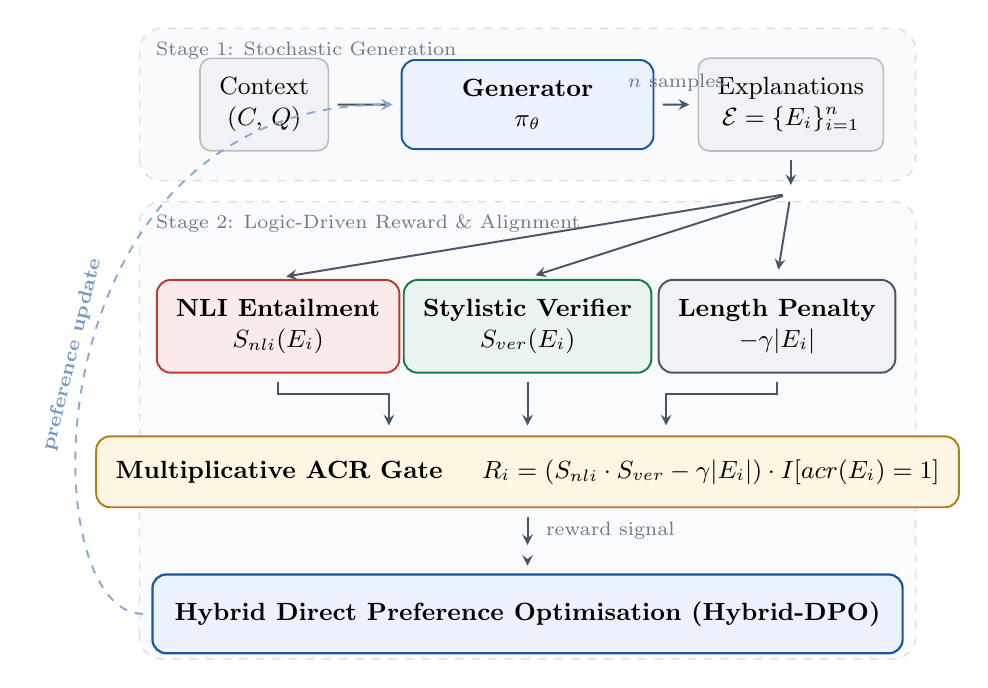
\begin{tikzpicture}[
    scale=0.88,
    >=stealth,
    % Core node styles
    iobox/.style={
        draw=NStroke, fill=NSlateFill,
        rounded corners=4pt, align=center,
        font=\small, inner sep=7pt, line width=0.6pt
    },
    modbox/.style={
        draw=#1, fill=#1Fill,
        rounded corners=5pt, align=center,
        font=\small\bfseries, inner sep=7pt,
        minimum height=1.0cm, minimum width=3.2cm,
        line width=0.7pt
    },
    gatebox/.style={
        draw=NGold, fill=NGoldFill,
        rounded corners=5pt, align=center,
        font=\small\bfseries, inner sep=7pt,
        minimum height=0.9cm, minimum width=7.2cm,
        line width=0.7pt
    },
    dpobox/.style={
        draw=NBlue, fill=NBlueFill,
        rounded corners=5pt, align=center,
        font=\small\bfseries, inner sep=8pt,
        minimum height=1.0cm, minimum width=9.0cm,
        line width=0.8pt
    },
    arr/.style={->, line width=0.7pt, color=NSlate, shorten >=3pt, shorten <=3pt},
    arrd/.style={->, line width=0.7pt, color=NBlue!50, dashed, shorten >=3pt, shorten <=3pt},
    steplabel/.style={font=\footnotesize\bfseries, color=NSlate},
    sublabel/.style={font=\scriptsize, color=NSlate!80}
]

%% -------------------------------------------------------
%% STAGE 1 background (subtle)
\draw[draw=NStroke!50, fill=NSlateFill!40, rounded corners=8pt, line width=0.5pt, dashed]
    (-5.6, 2.8) rectangle (5.6, 5.0);
\node[sublabel, anchor=north west] at (-5.5, 4.95) {Stage 1: Stochastic Generation};

%% STAGE 1: Input → Generator → Candidates
\node[iobox] (input) at (-3.8, 3.9) {Context\\$(C,\, Q)$};
\node[modbox=NBlue] (gen) at (0, 3.9) {Generator\\$\pi_{\theta}$};
\node[iobox] (cands) at (3.8, 3.9) {Explanations\\$\mathcal{E} = \{E_i\}_{i=1}^{n}$};

\draw[arr] (input) -- (gen);
\draw[arr] (gen) -- node[above, sublabel, yshift=1pt] {$n$ samples} (cands);

%% -------------------------------------------------------
%% STAGE 2 background
\draw[draw=NStroke!50, fill=NSlateFill!30, rounded corners=8pt, line width=0.5pt, dashed]
    (-5.6, -4.1) rectangle (5.6, 2.5);
\node[sublabel, anchor=north west] at (-5.5, 2.45) {Stage 2: Logic-Driven Reward \& Alignment};

%% Fan-out connector
\draw[arr] (cands.south) -- ++(0,-0.6) coordinate (fanout);
\draw[arr] (fanout) -- (-3.6, 1.4);
\draw[arr] (fanout) -- (0,   1.4);
\draw[arr] (fanout) -- ( 3.6, 1.4);

%% REWARD COMPONENTS
\node[modbox=NRed,   minimum width=3.0cm] (nli) at (-3.6, 0.7)
    {NLI Entailment\\$S_{\text{nli}}(E_i)$};
\node[modbox=NGreen, minimum width=3.0cm] (ver) at (0,    0.7)
    {Stylistic Verifier\\$S_{\text{ver}}(E_i)$};
\node[modbox=NSlate, minimum width=3.0cm] (len) at ( 3.6, 0.7)
    {Length Penalty\\$-\gamma |E_i|$};

%% Converge arrows
\draw[arr] (nli.south) -- ++(0,-0.3) -| (-2.0,-0.85);
\draw[arr] (ver.south) -- ++(0,-0.3) -- (0,-0.85);
\draw[arr] (len.south) -- ++(0,-0.3) -| ( 2.0,-0.85);

%% GATE
\node[gatebox] (gate) at (0, -1.4)
    {Multiplicative ACR Gate \quad
     $R_i = (S_{\text{nli}} \cdot S_{\text{ver}} - \gamma|E_i|)\cdot\mathbb{I}[\text{acr}(E_i)=1]$};

%% DPO
\draw[arr] (gate.south) -- node[right, sublabel, xshift=3pt] {reward signal} ++(0,-0.65) coordinate (mid);
\draw[arr] (mid) -- ++(0,-0.3);

\node[dpobox] (dpo) at (0, -3.45)
    {Hybrid Direct Preference Optimisation (Hybrid-DPO)};

%% FEEDBACK LOOP
\draw[arrd]
    (dpo.west)
    .. controls (-7.2, -3.45) and (-7.2, 3.9) ..
    (gen.west)
    node[midway, sloped, above, font=\scriptsize\bfseries, color=NBlue!60]
        {preference update};

\end{tikzpicture}
\caption{The \textbf{RLearner-LLM} framework. Stage~1 samples $n$ candidate explanations from the generator $\pi_\theta$. Stage~2 scores each candidate via three complementary signals—NLI entailment, a stylistic verifier, and a length penalty—gated by answer coverage (ACR) to suppress hallucinated responses. Preference pairs are then formed from the scored pool and used to update $\pi_\theta$ via Hybrid-DPO.}
\label{fig:hybrid_dpo}
\end{figure}

\section{Methodology}
\label{sec:methodology}

\subsection{First-Principles Derivation of the Hybrid Reward}
\label{sec:first_principles}

\paragraph{The RLHF Objective and Its Core Tension.}
The canonical RLHF objective~\cite{ouyang2022training} is:
\begin{equation}
\max_{\pi_\theta}\; \mathbb{E}_{y \sim \pi_\theta(y|x)}\bigl[r(x,y)\bigr] - \beta\,\text{KL}\bigl(\pi_\theta \,\|\, \pi_\text{ref}\bigr)
\label{eq:rlhf}
\end{equation}
where $\pi_\text{ref}$ is the supervised fine-tuned reference policy and $\beta$ controls how much the learned policy is allowed to deviate from it.
DPO~\cite{rafailov2023direct} derives the closed-form optimal policy
$\pi^*(y|x) \propto \pi_\text{ref}(y|x)\cdot\exp(r(x,y)/\beta)$ and reformulates the objective as a direct binary cross-entropy loss on preference pairs, eliminating the need for an explicit reward model.

The KL term in Eq.~\ref{eq:rlhf} is the structural source of the \textbf{alignment tax}: it regularises the policy toward $\pi_\text{ref}$, which was trained via maximum-likelihood estimation (MLE) on human-written text. MLE by definition maximises fluency and surface coherence. Any reward signal that competes with this fluency prior---such as a pure NLI entailment objective---must overcome the KL gradient pulling the policy back toward verbose, fluent-but-logically-weak outputs.
This tension is not an implementation artefact; it is a structural consequence of Eq.~\ref{eq:rlhf} that persists regardless of the DPO variant used.

\paragraph{Why Additive Reward Combination Fails.}
A natural response is the additive blend $R_\text{add}(E) = \alpha\,S_\text{NLI}(E) + (1-\alpha)\,S_\text{ver}(E)$, which embeds a logical \textbf{OR} assumption: high reward is achievable via high NLI \emph{or} high verifier score. Because the Alpaca-7B verifier consistently rewards fluent-but-logically-weak explanations, the additive form admits chosen pairs satisfying only the fluency component, pushing DPO toward the fluent attractor and \emph{amplifying} the alignment tax. Our ablation confirms this: additive Hybrid DPO reaches NLI $=0.1411$ on Cardiff, \textbf{below} the SFT baseline ($0.1959$); NLI-only DPO is similarly below ($0.1419$).

\paragraph{The Conjunctive Requirement: AND, Not OR.}
From first principles, a logically sound explanation $E$ of a multiple-choice answer must \emph{simultaneously} satisfy two conditions:
\begin{enumerate}
    \item \textbf{Necessary condition} (Answer Coverage): $E$ must reference the key concepts of the correct option.
    An explanation that does not mention the answer cannot logically entail it---this is a strict semantic prerequisite.
    \item \textbf{Sufficient condition} (Logical Entailment): Given that the answer concepts are present, $E$ must construct a valid reasoning path from those concepts to the correct option.
\end{enumerate}
These requirements are \textbf{conjunctive} (AND), not disjunctive (OR). The correct algebraic encoding of a conjunction is multiplication, not addition. We therefore define the Hybrid reward as:
\begin{equation}
R(E) = \bigl(w_\text{nli}\cdot S_\text{NLI}(E)\;\cdot\; w_\text{ver}\cdot S_\text{ver}(E)\;-\;\gamma\cdot\ell_\text{norm}(E)\bigr)\cdot\mathbf{1}\bigl[\mathrm{ACR}(E)\geq\theta\bigr]
\label{eq:hybrid_reward}
\end{equation}
where $\mathbf{1}[\cdot]$ is a hard indicator enforcing the necessary condition, the multiplicative product $S_\text{NLI}\cdot S_\text{ver}$ encodes the conjunctive sufficient condition, and $\gamma\cdot\ell_\text{norm}$ removes a known length-based confounder (described below).

\paragraph{ACR Gate and Length Penalty.}
\label{sec:length_norm}
The indicator $\mathbf{1}[\mathrm{ACR}(E){\geq}\theta]$ zeroes out any explanation that fails to cover the answer keywords, removing answer-evasive pairs by construction (a non-hypothetical failure mode---Appendix~\ref{sec:failure_mode_appendix} shows answer evasion in $12$--$37\%$ of SFT outputs across domains). The penalty $-\gamma\,\ell_\text{norm}(E)$ corrects a known length confounder: both $S_\text{NLI}$ and $S_\text{ver}$ correlate positively with output length, so without correction the DPO gradient drifts toward verbosity, reinstating a length-driven form of the alignment tax.

\subsection{Preference Pair Construction}
\label{sec:pref_construction}

Given $n$ candidate explanations $\{E_i\}_{i=1}^n$ sampled from $\pi_\theta$ for a question-context pair $(C, Q)$, we score each candidate with $R(E_i)$ via Eq.~\ref{eq:hybrid_reward}. Pairs $(E_i, E_j)$ with $R(E_i) > R(E_j) + \Delta$ are retained as (chosen, rejected) pairs, where $\Delta \geq 0.1$ is a minimum score gap that ensures the signal-to-noise ratio of the preference label. This yields a dataset $\mathcal{D}_\text{pref} = \{(x_k, y_k^+, y_k^-)\}_{k=1}^K$ used to train Hybrid-DPO.

\subsection{Hybrid-DPO Training Objective}
\label{sec:hybrid_dpo}

The Hybrid-DPO objective follows the standard DPO formulation~\cite{rafailov2023direct} but is trained on $\mathcal{D}_\text{pref}$ constructed with the Hybrid reward (Eq.~\ref{eq:hybrid_reward}):
\begin{equation}
\mathcal{L}_\text{DPO}(\pi_\theta) = -\mathbb{E}_{(x,y^+,y^-)\sim\mathcal{D}_\text{pref}}\!\left[\log\sigma\!\left(\beta\!\left(\log\frac{\pi_\theta(y^+|x)}{\pi_\text{ref}(y^+|x)} - \log\frac{\pi_\theta(y^-|x)}{\pi_\text{ref}(y^-|x)}\right)\right)\right]
\label{eq:dpo_loss}
\end{equation}
Because every chosen example $y^+$ in $\mathcal{D}_\text{pref}$ is guaranteed to pass the ACR gate and to outscore its rejected counterpart on the conjunctive NLI$\times$Verifier product, the gradient of $\mathcal{L}_\text{DPO}$ consistently points toward higher logical entailment. This is the mechanism by which the Hybrid reward breaks the fluency attractor that causes alignment tax in additive variants.

\paragraph{Implementation notes.}
Two base models in this study require non-default LoRA target selection. Qwen3-8B applies RMSNorm to $q,k$ after the projection reshape, so LoRA adapters on \texttt{q\_proj}/\texttt{k\_proj} would corrupt that path; we restrict its targets to \texttt{v\_proj}, \texttt{o\_proj}, and the three MLP projections. Gemma 4 E4B-it ships as a multimodal \texttt{Gemma4ForConditionalGeneration} checkpoint whose text-tower weights live under \texttt{model.language\_model.*}; we therefore load that class explicitly and use a full-path LoRA target regex that matches exactly the $258$ plain \texttt{nn.Linear} attention/MLP projections in the text tower (full pattern in Appendix~\ref{sec:impl_notes_appendix}). At inference, the DPO adapter must be composed on top of the SFT-merged base ($\text{base}\to\text{apply SFT}\to\text{merge}\to\text{apply DPO}\to\text{merge}$), since the DPO delta was trained relative to that reference point.
